\documentclass[notitlepage, a4paper, 11pt]{article}

\usepackage{geometry}
\geometry{
	a4paper,
	total={170mm,257mm},
	left=20mm,
	top=20mm,
}
\usepackage{ gensymb }
\usepackage{wrapfig}
\usepackage{xcolor}
\usepackage{graphicx}
\usepackage{amsmath}
\usepackage{listings}
\usepackage{xcolor}
\usepackage{minted}
\usepackage{tikz}
\usepackage[european resistors]{circuitikz}
\usepackage{caption}
\usepackage{subcaption}
\usepackage{hyperref}
\hypersetup{
	pdfborder = false,
	colorlinks=true,
	linkcolor=black,
	filecolor=black,      
	urlcolor=blue,
	pdftitle={Overleaf Example},
	pdfpagemode=FullScreen,
}
\title{Frequency Response Measurements\\
	\large Laboratory IV}
\author{Patrycja Nazim, Adrian Król, Gabriel Ćwiek, Kamil Chaj}
\date{}

\begin{document}
	\maketitle
	\section{Goal of the exercise}
	\section{Frequency response}
	\section{Course of measurements}
	\begin{figure}[H]
		\centering
			\begin{subfigure}{0.35\textwidth}
				\centering
				\begin{circuitikz}[scale = 0.7, transform shape]
					\draw (0,0) node[bnc](B1) {CON11}
					to[R, l=$R_{11}$, a=1.5k$\Omega$] (3,0)
					to[C, l=$C_{11}$, a=47nF] (3,-2)
					node[ground] {}
					;
					\draw (3,0) 
					to[short] (4.5,0)
					node[bnc, xscale=-1](B2){\scalebox{-1}[1]{CON12}}
					;
					\draw node[ground] at (B1.shield) {};
					\draw node[ground] at (B2.shield) {};
				\end{circuitikz}
				\caption{RC low-pass filter}
			\end{subfigure}
			\hfill
			\begin{subfigure}{0.50\textwidth}
				\centering
				\begin{circuitikz}[scale = 0.7, transform shape]
					\node [bnc] at (0,0) (CON41) {CON41};
					\draw (CON41.hot) to[short, -*]
					(1,0) -- (3,0) to[nopb, l_=JP43] (4,0);
					\draw (1,0) -- (1,-2) to[R, l2=$R_{42}$ and $1.1k\Omega$, l2 halign=c, l2 valign=b] (3,-2)
					to[nopb, l_=JP42] (4,-2) -- (4, 0);
					\draw (1,-2) -- (1,-4) to[R, l2=$R_{41}$ and $3.3k\Omega$, l2 halign=c, l2 valign=b] (3,-4)
					to[nopb, l_=JP41] (4,-4) -- (4, -2);
					\draw (4,0) to[short, -*] (5,0)
					to[C, l2=$C_{41}$ and 33nF, l2 halign=c, l2 valign=c] (5,-2) 
					to[L, l2=$L_{41}$ and 10mH, l2 halign=c, l2 valign=c] (5,-4) node[ground] {};
					\draw (5, 0) to (6, 0) node[bnc, xscale=-1, anchor=zero](CON42){\ctikzflipx{CON42}};
				\end{circuitikz}
				\caption{III-order low-pass filter}
			\end{subfigure}
			\centering
			\begin{subfigure}{\textwidth}
				\centering
				\begin{circuitikz}
					\ctikzset{bipoles/length = 10mm}
					\ctikzset{font = \tiny}
					\node [bnc] at (0, 0)(CON1) {CON31};
					\node [bnc, xscale=-1] at (8, 0)(CON2) {\ctikzflipx{CON32}};
					\draw (CON1.hot) -- (1.5, 0)
					to[C, l2=$C_{31}$ and 1$\mu$F, l2 halign=c, l2 valign=a] (1.5, -2) node[tlground]{};
					\draw (1.5, 0) -- (3, 0)
					to[C, l2=$C_{32}$ and 330nF, l2 halign=c, l2 valign=c] (3, -2) node[tlground]{};
					\draw (3, 0)
					to[L, l2=$L_{31}$ and 680$\mu$H, l2 halign=c, l2 valign=c] (4.5, 0)
					to[C, l2=$C_{34}$ and 330nF, l2 halign=c, l2 valign=c] (4.5, -2) node[tlground]{};
					\draw (4.5, 0) -- (6, 0)
					to[C, l2=$C_{34}$ and 330nF, l2 halign=c, l2 valign=c] (6, -2) node[tlground]{};
					\draw (6, 0) -- (CON2.hot);
					\draw (7.5, 0) 
					to[nopb] (7.5, -1)
					to[R, l2^=$R_{31}$ and 51$\Omega$, l2 halign=c, l2 valign=c, bipoles/length = 8mm] (7.5, -2) node[tlground]{};
				\end{circuitikz}
				\caption{Resonant RLC circuit}
			\end{subfigure}
			\caption{Measured circuits}
	\end{figure}
	
	\section{Data processing}
	\begin{wrapfigure}{r}{0.4\textwidth}
		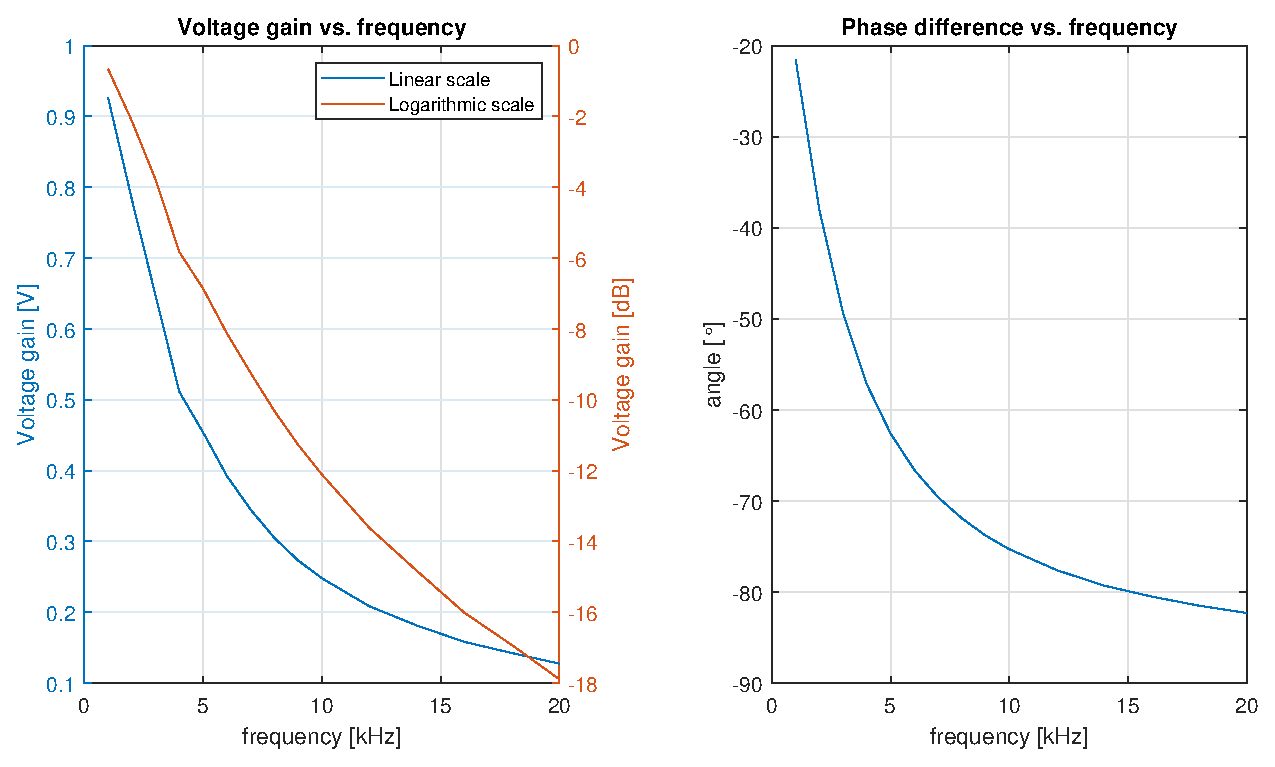
\includegraphics[width=0.4\textwidth]{../Matlab/img/11.eps}
		\caption{Example}
		\label{fig:example}
	\end{wrapfigure}
	
	Source code for this section can be found in Appendix \ref{sec:appendix}
	
	First step in finding amplitude-frequency characteristics was calculating gain in Volts
	
	\begin{equation}
		\text{Voltage gain [V]} = \dfrac{V_{\text{CON2}}}{V_{\text{CON1}}}
	\end{equation}
	
	then we calculated voltage gain in decibels
	
	\begin{equation}
		\text{Voltage gain [dB]} = 20 \log_{10}(V_{\text{gain}})
	\end{equation}
	
	Voltage gain is on the left plot in figure \ref{fig:example}, vertical blue axis represents scale in volts and orange axis decibel scale.
	
	Phase-frequency characteristics didn't require any calculation and is simply plotted on the right plot in figure \ref{fig:example}.
	
	\section{Characteristics analysis}
	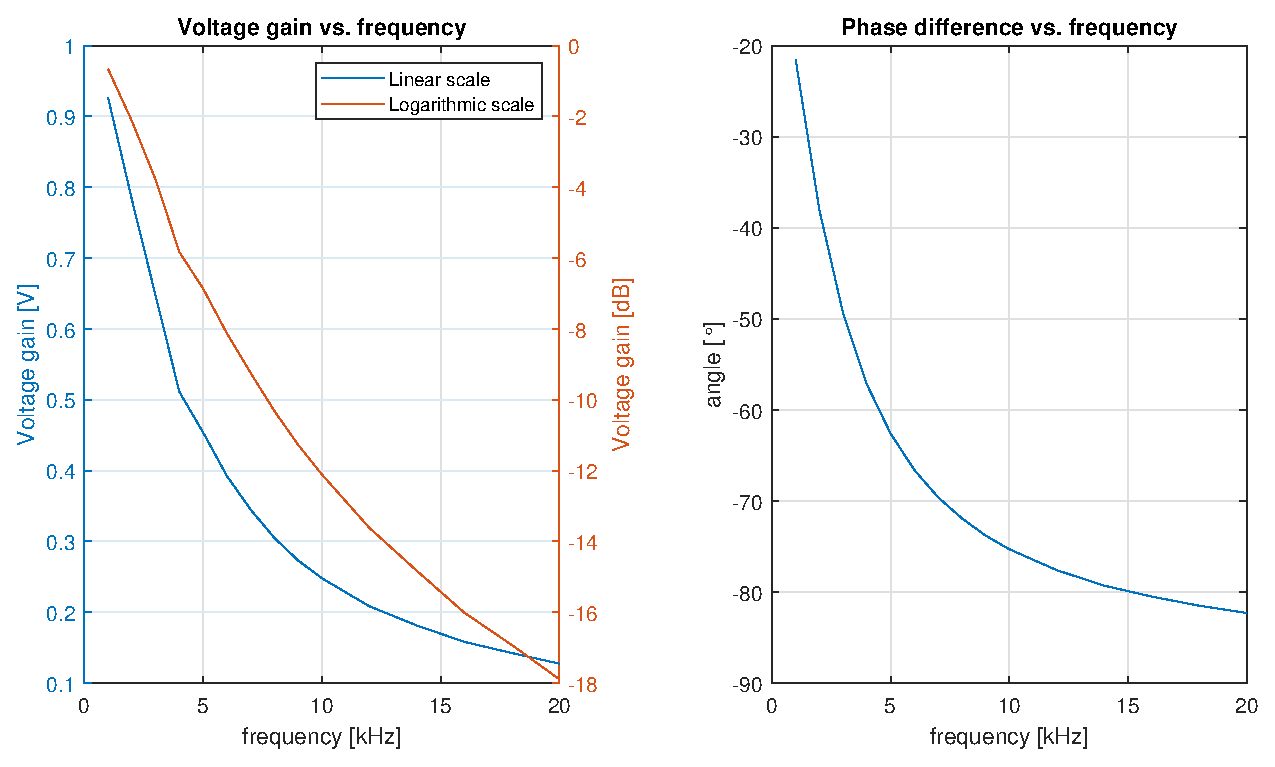
\includegraphics[width=\textwidth]{../Matlab/img/11.eps}
	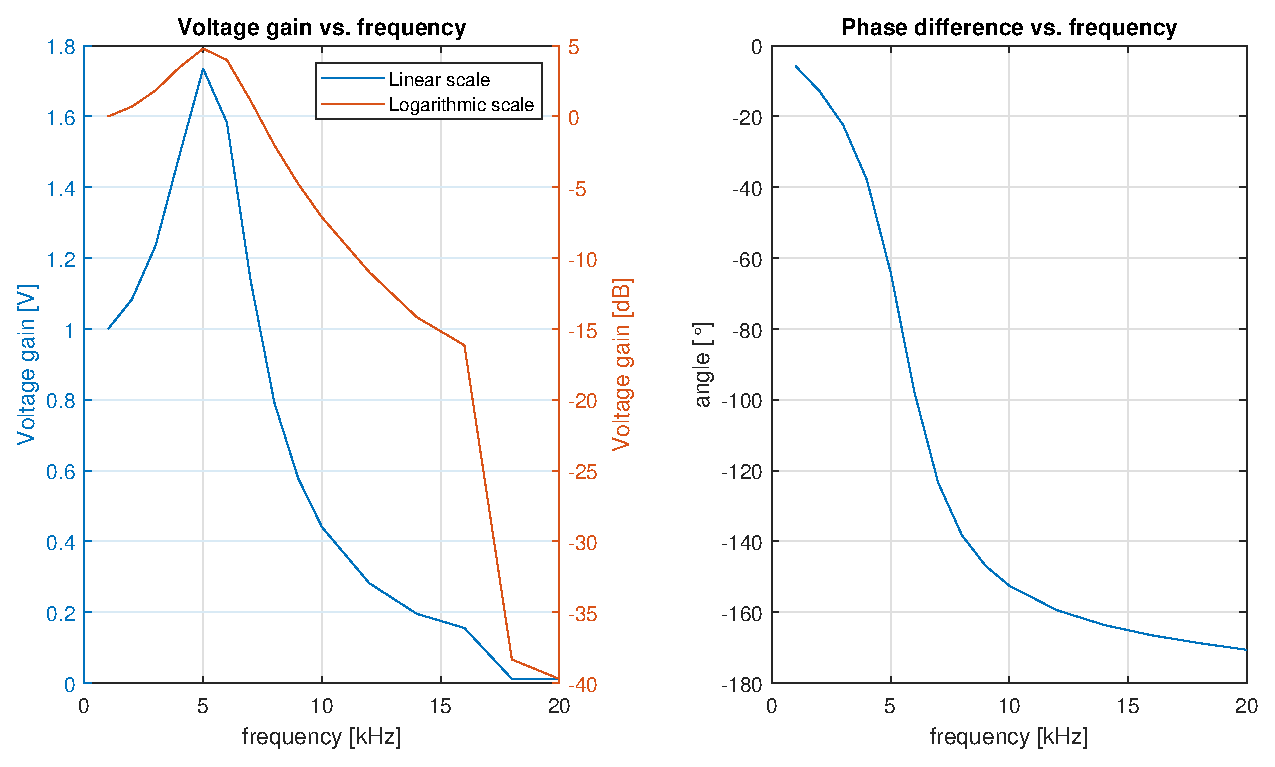
\includegraphics[width=\textwidth]{../Matlab/img/12.eps}
	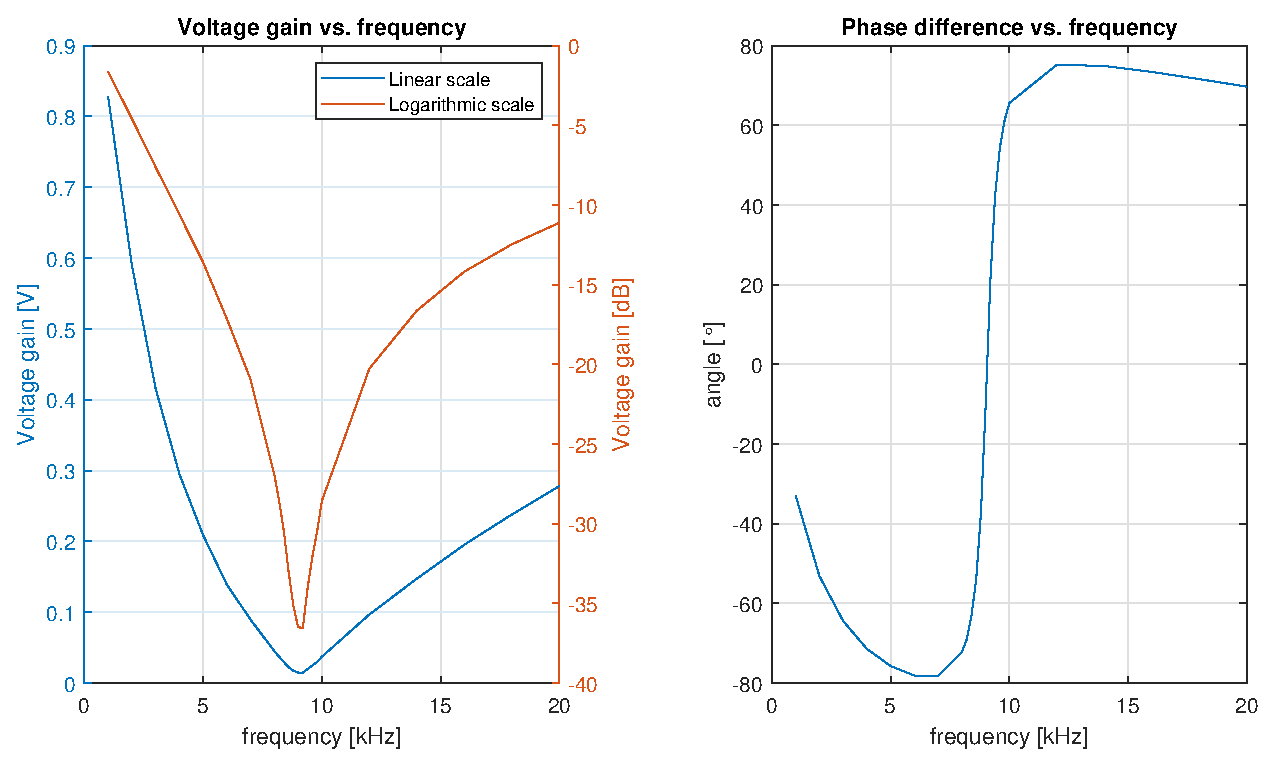
\includegraphics[width=\textwidth]{../Matlab/img/131.eps}
	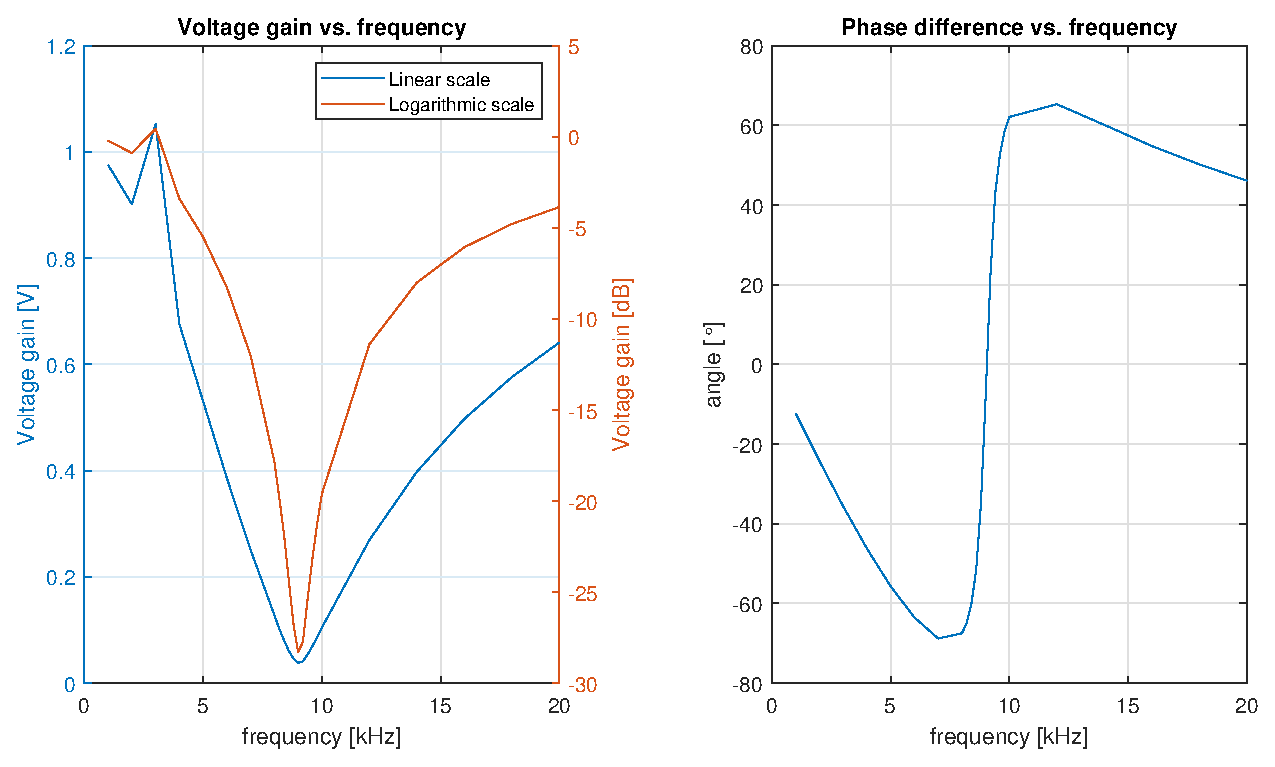
\includegraphics[width=\textwidth]{../Matlab/img/132.eps}
	\section{Conclusions}
	
	
	\newpage
	\appendix
	\section{Appendix}\label{sec:appendix}
\end{document}